\documentclass[aps,reprint]{revtex4-1}
% Engine-specific settings
% Detect pdftex/xetex/luatex, and load appropriate font packages.
% This is inspired by the approach in the iftex package.
% pdftex:
\ifx\pdfmatch\undefined
\else
    \usepackage[T1]{fontenc}
    \usepackage[utf8]{inputenc}
\fi
% xetex:
\ifx\XeTeXinterchartoks\undefined
\else
    \usepackage{fontspec}
    \defaultfontfeatures{Ligatures=TeX}
\fi
% luatex:
\ifx\directlua\undefined
\else
    \usepackage{fontspec}
\fi
% End engine-specific settings
\usepackage[english]{babel}
\usepackage{csquotes}
% \usepackage[backend=biber, sortcites]{biblatex}
\usepackage{url}
\usepackage{textcomp}
\usepackage[usenames,dvipsnames,svgnames, table]{xcolor}
\usepackage[font={scriptsize}]{caption}
\usepackage{amsmath} \usepackage{amsthm} \usepackage{amsfonts}
\usepackage{amssymb}
\usepackage{enumerate}
\usepackage{tikz} \usepackage{float}
\usepackage[procnames]{listings}
\usepackage{pstool} \usepackage{pgfplots}
\usepackage{wrapfig} \usepackage{graphicx} \usepackage{epstopdf}
\usepackage{afterpage}
\usepackage{physics}
\usepackage{multirow}
\usepackage{gensymb}
\usepackage{algorithm}
\usepackage{microtype}
\usepackage[noend]{algpseudocode}
\usepackage{xcolor,colortbl}
\usepackage{microtype}
\usepackage{geometry}
\usepackage{hyperref}
\usepackage{graphicx}
\usepackage{caption}
\usepackage{subcaption}
\usepackage{lipsum}
% \usepackage{pythontex}
% \usepackage{authblk}
\usepackage{nth}
\usepackage{siunitx}
% \usepackage[toc,page]{appendix}
\floatstyle{plaintop}
\restylefloat{table}

% SET LISTING STUFF (FRED)
\definecolor{dkgreen}{rgb}{0,0.6,0}
\definecolor{dred}{rgb}{0.545,0,0}
\definecolor{dblue}{rgb}{0,0,0.545}
\definecolor{lgrey}{rgb}{0.9,0.9,0.9}
\definecolor{gray}{rgb}{0.4,0.4,0.4}
\definecolor{darkblue}{rgb}{0.0,0.0,0.6}
\lstdefinelanguage{cpp}{
      backgroundcolor=\color{lgrey},
      basicstyle=\footnotesize \ttfamily \color{black} \bfseries,
      breakatwhitespace=false,
      breaklines=true,
      captionpos=b,
      commentstyle=\color{dkgreen},
      deletekeywords={...},
      escapeinside={\%*}{*)},
      frame=off,
      language=C++,
      keywordstyle=\color{purple},
      morekeywords={BRIEFDescriptorConfig,string,TiXmlNode,DetectorDescriptorConfigContainer,istringstream,cerr,exit},
      identifierstyle=\color{black},
      stringstyle=\color{blue},
      % numbers=left,
      % numbersep=5pt,
      numberstyle=\tiny\color{black},
      rulecolor=\color{black},
      showspaces=false,
      showstringspaces=false,
      showtabs=false,
      stepnumber=1,
      tabsize=5,
      title=\lstname,
    }

% Custom commands
\newcommand{\unit}[1]{\:\mathrm{#1}}
\newcommand{\noref}[1]{\hyperref[#1]{\ref*{#1}}}
\newcommand{\nonref}[1]{\hyperref[]{\ref*{#1}}}
\newcommand\blankpage{%
  \null
  \thispagestyle{empty}%
  \addtocounter{page}{-1}%
  \newpage}

% Default fixed font does not support bold face
\DeclareFixedFont{\ttb}{T1}{txtt}{bx}{n}{7} % for bold
\DeclareFixedFont{\ttm}{T1}{txtt}{m}{n}{7}  % for normal

\newcommand\numberthis{\addtocounter{equation}{1}\tag{\theequation}}
\DeclareCaptionFont{white}{\color{white}}
\DeclareCaptionFormat{listing}{\colorbox{gray}{\parbox{\columnwidth}{#1#2#3}}}
\captionsetup[lstlisting]{format=listing,labelfont=white,textfont=white}


% Biber for references
% \bibliographystyle{aipauth4-1}

\begin{document}
\sisetup{detect-all}
\title{Numerical approaches to solving Schrödinger's equation for
two electrons in an external oscillator potential with C++ and Julia}
\author{Erlend Lima}
\author{Frederik J. Mellbye}
% \author{Aram Salihi}
\affiliation{University of Oslo, Oslo, Norway \\ Source code available at: \url{https://github.com/Caronthir/FYS3150/tree/master/Project2}}
\date{\today}

\begin{abstract}
  This is really abstract. So abstract it is spooky :O
\end{abstract}
\maketitle
\tableofcontents
\makeatletter
\let\toc@pre\relax
\let\toc@post\relax
\makeatother

\newpage

% % Get all of the data from the script into a dictionary
% \begin{pycode}
% from subprocess import Popen, PIPE
% from latextools import untag_all
% p = Popen(['python', '../analysis/analyze.py', '../cpp'],
% stdout=PIPE, stderr=PIPE)
% output, err = p.communicate()
% data = output.decode('utf8')
% latex_data = untag_all(data)
% \end{pycode}
%
% \begin{table}[ht]
%   \centering
%   \pyc{print(latex_data['error_table'])}
%   \caption{Summary of the errors}
%   \label{tab:error}
% \end{table}
%
% \begin{figure}[ht]
%   \centering
%   
\includegraphics[scale=0.5]{figures/function.eps}
%   \caption{\label{fig:general} Caption}
% \end{figure}
\section{Introduction}
\label{sec:introduction}
Eigenvalue problems occur frequently in mathematics and science. Many problems
are on or can be re-written to the form
\begin{align*}
  A \mathbf{x} = \lambda \mathbf{x}
\end{align*}
For matrices where $n \geq 5$ there is
no general analytical procedure to obtain the roots of the characteristic polynomial, by the
Abel-Ruffini theorem. In most situations the eigenvalue problems have much
larger matrices, on the order \(n\sim 10\), and numerical algorithms are needed to solve the problems. In
this paper, the direct Jacobi rotation and iterative Lanczos method
are investigated.The algorithm accuracies are compared to each other and the
built-in eigenvalue solvers in Armadillo and Julia.

The methods are used to solve Schrödinger's equation for two electrons in a
three-dimensional harmonic oscillator potential, which can be reformulated into
an eigenvalue problem through scaling and mathematical manipulations. The
energy eigenvalues and associated eigenstates are then obtained by Jacobi's method,
and compared to known analytic solutions.

The study of electrons confined in a potential is a highly active research field,
because of the possible nano-medical applications, and in the development of semi-conductors
and quantum computers.
\section{Theory}
\label{sec:theory}
\subsection{Jacobi's rotation algorithm}
The general idea of Jacobi's algorithm is rather straightforward. Finding the
eigenvalues of any matrix is hard, but finding the eigenvalues of a diagonal
matrix is trivial. A matrix \(A\) is converted to an approximately a diagonal
matrix through a series of orthogonal matrix transformations on the form:
\begin{align*}
  T = S^T A S
\end{align*}
where $S$ is a rotation matrix. This amounts to rotating the rotating the matrix
around hyperplanes in such a way that the off-diagonal elements are reduced to
fall beneath some threshhold.
Since eigenvalues are preserved under similarity
transformations, the eigenvalues of \(A\) can be read off the diagonal of a
sufficiently diagonalized matrix. For a more detailed description, see REF.

\subsubsection{Jacobi sweep variations}
Cyclic jacobi (systematically cycle over all elements) and classic Jacobi (the one we are using, find max offdiagonal element)
\subsection{The Harmonic Oscillator}
\label{sec:harmonic}
In the words of Richard Feynman, ``every potential can be reduced to a
combination of harmonic oscillators'' REF. The radial part of Schrödinger's
equation describing an electron in an harmonic oscillator is
\begin{equation}
  \label{eq:schroedinger}
  -\frac{\hbar^{2}}{2m} \left( \frac{1}{r^{2}}\dv{r}r^{2}\dv{r} - \frac{l(l+1)}{r^{2}} \right)R(r) + V(r)R(r) = ER(r)
\end{equation}
with potential
\begin{equation*}
  V(r) = \frac{1}{2}mω^{2}r^{2}
\end{equation*}
and energies
\begin{equation*}
  E_{nl} = \hbar\omega\left( 2n+l+\frac{3}{2} \right)
\end{equation*}
with \(n=0,1,2,\ldots\) and \(l = 0,1,2,\ldots\)

\eqref{eq:schroedinger} can be scaled and rewritten to a more practical form:

\begin{equation}
  \label{eq:scaledschroedinger}
  -\dv[2]{\rho}u(\rho)+\rho^{2}u(\rho) = \lambda u(\rho)
\end{equation}
see REF for a more detailed derivation. To solve this equation numerically,
\(\dv[2]{u}{\rho}\) is computed as
\begin{equation*}
  \dv[2]{u}{\rho} \simeq \frac{u(\rho+h)-2u(\rho)+u(\rho-h)}{h^{2}} + \mathcal{O}(h^{2})
\end{equation*}
where \(h\) is the step size.
bla bla bla
\section{Method}
\label{sec:method}

\subsection{Solving the Hamiltonian}
The Hamiltonian solved here describes two electrons trapped in an harmonic oscillator with
two different types of potential. In the first case, only the Coulomb force is
acting on the electron, while in the second, the electrons also feel a repulsive
force from each other.

To find the wave functions describing the position of the electrons, the matrix
described above in REF is set up for some values \(\rho_{\text{min}},
\rho_{\text{max}}, N\) and \(\omega_{r}\).
\subsection{Choice of $\omega_r$ to analyze}
\subsection{Choosing an appropriate value for infinity}
\subsection{Choice of step size}
\subsection{Multiple programming languages}
Implementering i Julia og C++. Trening og god måte å verifisere korrekt implementasjon.
\subsection{Unit tests}
Unit tests were implemented to verify that the implemented functions behave
as intended, and that this behaviour is preserved through changes to the programs.
\subsubsection{Correct maximum offdiagonal element}
\subsubsection{Jacobi's method on $3 \times 3$ matrix with known eigenvalues}
\subsubsection{Preservation of dot product and orthogonality?? Skal vi ta denne?}
\section{Results}
\label{sec:results}

\subsection{The Algorithm}
\label{sec:algorithm}

As the code was written on both Python+C++ and Julia, there were two sets of
results. Since all of the results agree, only one set of results is included.
The exception to this is the algorithm itself, which although equivalent, behave
a bit differently.

Figure~\ref{fig:juliatiming} compares the time it takes for the handwritten
Jacobi algorithm to find to eigenvalues of an \(N\times N\)-matrix, versus the
time it takes for the standard library methods to do the same. The Jacobi method
is written in both Julia and C++, while the standard Julia method and Armadillo
method are used as comparison. Only the memory consumption in Julia is measured
as C++ provides no easy way to measure this.

\begin{figure}[ht]
  \centering
  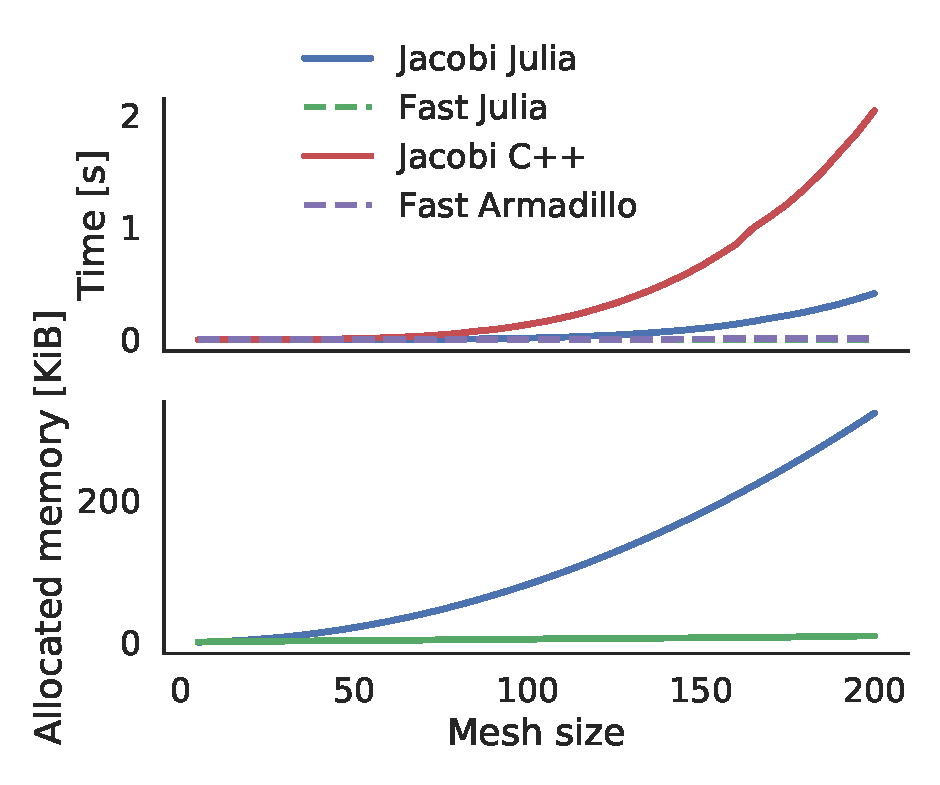
\includegraphics[width=\columnwidth]{figures/juliatime.eps}
  \caption{\label{fig:juliatiming} Time and amount of memory required to get the eigenvalues of an
    \(N\times N\)-matrix for the custom Jacobi method versus library methods. In
  the upper plot, the green dashed line of Julia's eigenvalue solver is hidden
  by the overlaying Armadillo's purple dashed line.}
\end{figure}

The number of similarity transforms needed to make all off-diagonal elements
less than \(\varepsilon=10^{-10}\) as \(N\) grows is plotted in
figure~\ref{fig:juliaiterations}.

\begin{figure}[ht]
  \centering
  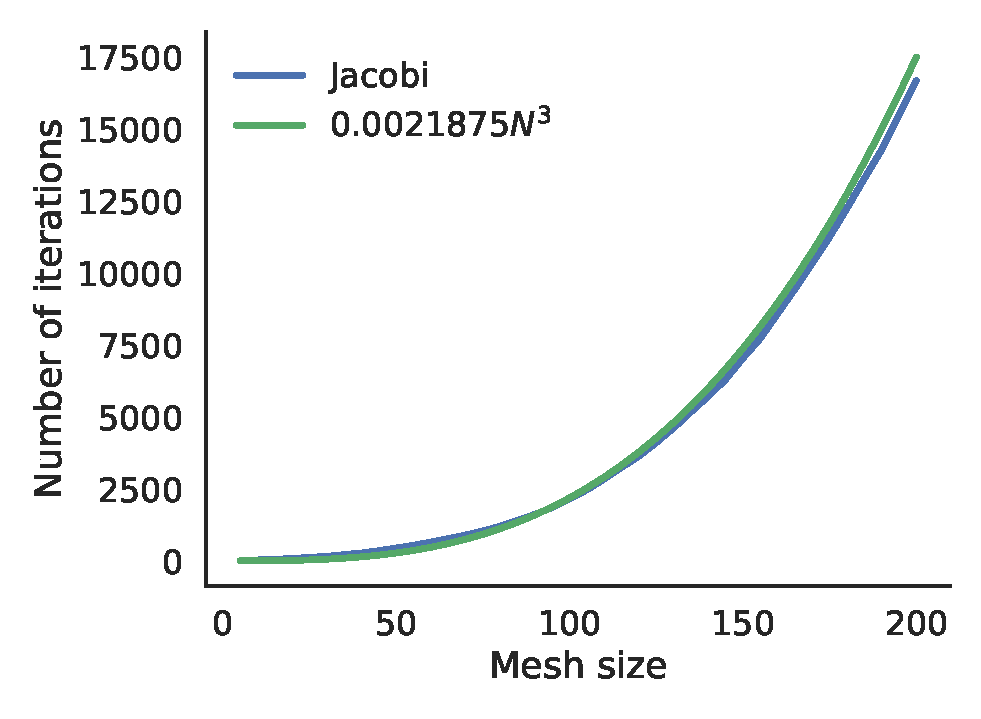
\includegraphics[width=\columnwidth]{figures/iterations.eps}
  \caption{\label{fig:juliaiterations} Number of iterations, or similarity
    transforms, needed to make all off-diagonal elements less than \(10^{-10}\).}
\end{figure}

\subsection{Solution of the Hamiltonian}
\label{sec:hamiltonsol}

\begin{figure}[ht]
  \centering
  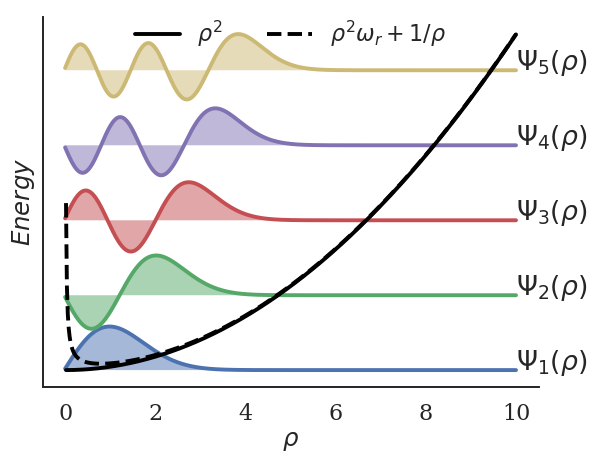
\includegraphics[width=\columnwidth]{figures/wavefunctions.png}
  \caption{\label{fig:wavefunctions} A visualization of the potentials and the
    corresponding wave functions for different eigenstates. The graphs have
    arbitrary scales, but have the same values of \(\rho\). The wavefunctions
    correspond to
    the first four bound eigenstates of the potential \(V=\rho^{2}\).}
\end{figure}



\begin{figure}[ht]
  \centering
  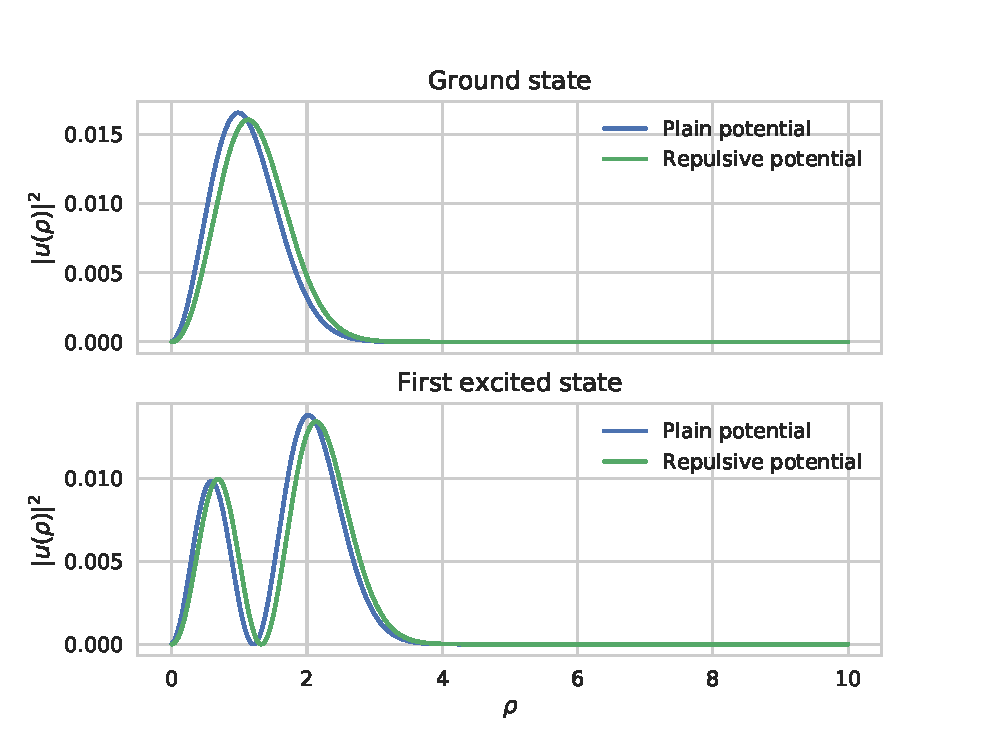
\includegraphics[width=\columnwidth]{figures/excitation.eps}
  \caption{\label{fig:excitation} Comparison of the probability of finding the
    electron at certain positions \(rho\) in the ground state (top) and first
    excited state (bottom) for both the Coulomb potential and repulsive potential.}
\end{figure}


\begin{figure}[ht]
  \centering
  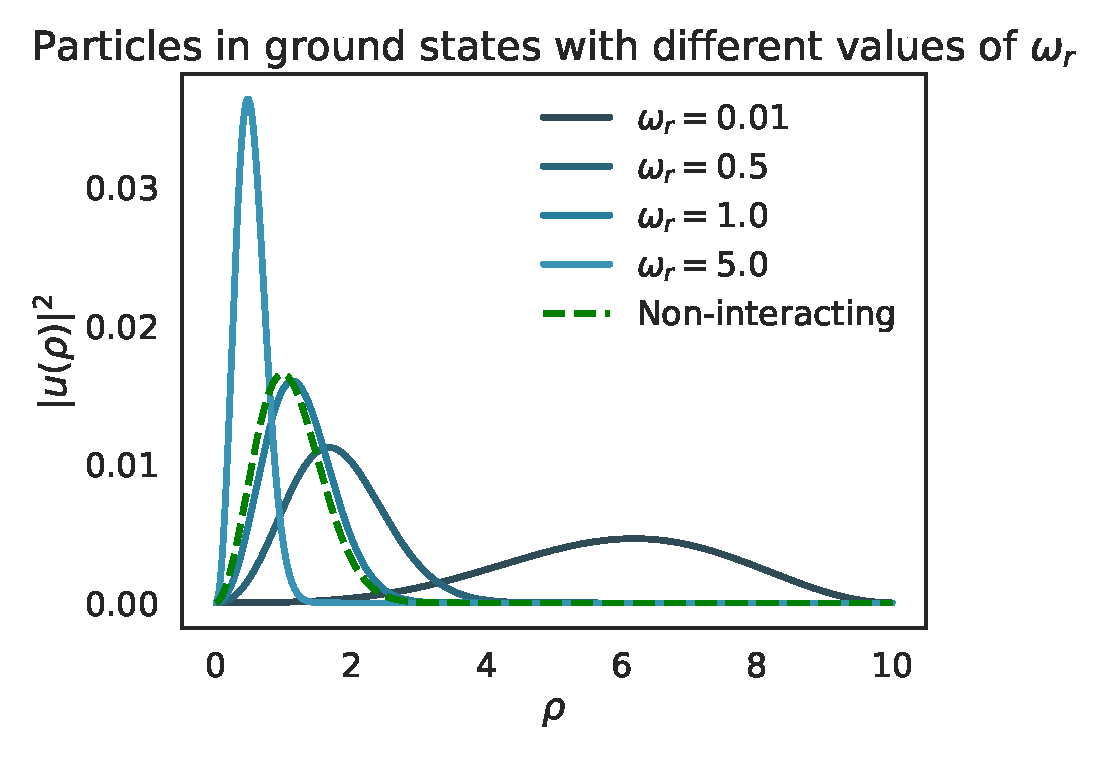
\includegraphics[width=\columnwidth]{figures/omegas.eps}
  \caption{\label{fig:omegas} Probabilities of the position of the electron when
  the repulsive potential is present.}
\end{figure}

\section{Discussion}

\subsection{The Algorithm}
Viewing figure~\ref{fig:juliatiming}, it is abundantly clear that the standard
library methods of both Julia and Armadillo are far superior to the custom
Jacobi methods, being both quicker and using less memory. More interestingly,
the Jacobi method written in Julia is quicker than the method written in C++.
The reason for this is unknown.

The Jacobi method takes considerably longer as the mesh size increases. From
figure~\ref{fig:juliaiterations} , the time needed grows approximately as
\(2.2\cdot 10^{-3}N^{3}\), at least as \(0\leq N \leq 200\). This renders
Jacobi's method completely useless at sufficiently large \(N\)s.

\subsection{Non-interacting case}
\subsection{Interacting case}
\label{sec:discussion}
\section{Conclusion}
\label{sec:conclusion}
\bibliography{references}
\blankpage
\appendix
\section{Proof of preservation of orthogonality and dot product for unitary transformations}
A unitary transformation preserves orthogonality and the dot product. To see
this, consider an orthogonal basis \(\{\vb{v}_{i}\}\) and an unitary
transformation \(U\). Defining \(\vb{w}_{i}=U\vb{v}_{i}\), the dot product can
be computed as
\begin{align*}
  \vb{w}_{i}\vdot \vb{w}_{j} &= \vb{w}_{i}\vb{w}_{j}^{T}\\
                             &= \left( U\vb{v}_{i} \right)\left( U\vb{v}_{j} \right)^{T}\\
                             &= U\vb{v}_{i}\vb{v}_{j}^{T}U^{T}\\
                             &= U\delta_{ij}U^{T}\\
                             &= \delta_{ij}UU^{T}\\
                             &= \delta_{ij}
\end{align*}
where the last step follows since \(U\) is unitary.
\blankpage
\end{document}

% Local Variables:
% TeX-engine: luatex
% End:
